\documentclass[12pt]{article}
\usepackage{graphicx}
\usepackage{subcaption}
\usepackage{float}
\usepackage{hyperref}

\title{EE236: Experiment 13\\
Characterising an Unknown Device}

\author{Aaron John Sabu, 170070050}

\begin{document}
\maketitle

\section{Aim of the experiment}

The experiment aims to realise the I-V Characteristics of an Unknown Device/Circuit and hence identify te circuit. Prior to this, the I-V Characteristics of a Bipolar Junction Transistor will be calculated. 

\section{Observations and Inferences}

\subsection{Bipolar Junction Transistor}

\begin{figure}[H]
	\centering
	\includegraphics[width = 0.63\linewidth, trim = {0 0 0 0}, clip]{Part1.png}
	\caption{\( I_C-V_{CE} \) Characteristics for Varying \( I_B \)}
\end{figure}
The previous plot for the \( I_C-V_{CE} \) characteristics was created using the following data obtained in the lab:
\begin{center}
 \begin{tabular}{|| c | c | c | c | c | c ||} 
 \hline
 \hline
 \multicolumn{2}{||c|}{\( I_B = 100\ \mu A \)} & \multicolumn{2}{c||}{\( I_B = 148.6\ \mu A \)} \\
 \hline
 \hline
\( V_{CE} \) & \( I_{C} \) & \( V_{CE} \) & \( I_{C} \) \\ [0.25ex] 
 \hline\hline
 \hline 
0.00 & 0.00 & 0.000 & 0.00 \\ \hline
0.05 & 3.29 & 0.056 & 3.65 \\ \hline
0.10 & 9.67 & 0.120 & 13.04 \\ \hline
0.13 & 13.98 & 0.156 & 18.48 \\ \hline
0.18 & 18.52 & 0.205 & 23.38 \\ \hline
0.22 & 20.33 & 0.281 & 26.53 \\ \hline
0.25 & 21.08 & 0.308 & 27.06 \\ \hline
0.28 & 21.59 & 0.323 & 27.41 \\ \hline
0.32 & 22.32 & 0.349 & 27.82 \\ \hline
0.38 & 23.06 & 0.411 & 28.83 \\ \hline
0.42 & 23.59 & 0.467 & 29.64 \\ \hline
0.45 & 24.00 & 0.512 & 30.23 \\ \hline
0.49 & 24.50 & 0.558 & 30.95 \\ \hline
0.54 & 25.16 & 0.660 & 32.37 \\ \hline
0.69 & 26.90 & 0.821 & 34.45 \\ \hline
0.82 & 28.29 & 0.978 & 36.35 \\ \hline
1.00 & 30.03 & 1.200 & 38.90 \\ \hline
1.18 & 31.49 &  -  &  -  \\ \hline
\end{tabular}
\end{center}

The equations obtained for the linear region of the plots are given below. From these, we may calculate the Early voltage (x-intercept):
\begin{center}
 \begin{tabular}{|| c | c || c ||} 
 \hline
 \hline
\( I_B \) & Equation of the plot & Early voltage \\ [0.25ex] 
 \hline\hline
 \hline 
\( 100\ \mu A \) & \( y = 10.182 x + 19.719 \) & -1.937 V \\ \hline
\( 148.6\ \mu A \) & \( y = 12.355 x + 24.184 \) & -1.957 V \\ \hline
\end{tabular}
\end{center}

\subsection{Unknown Device}

The given device consisted of three pins which we identified in the following manner:
\begin{enumerate}
	\item Terminal 1 - Long Red Wire
	\item Terminal 2 - Short Red Wire
	\item Terminal 3 - Blue Wire
\end{enumerate}
Hence we obtained the following readings where the first mentioned terminal was placed positive:
\begin{center}
 \begin{tabular}{|| c | c || c | c || c | c ||} 
 \hline
 \hline
 \multicolumn{2}{||c|}{Terminal 1 / Terminal 3} & \multicolumn{2}{c||}{Terminal 2 / Terminal 3} & \multicolumn{2}{c||}{Terminal 1 / Terminal 2} \\
 \hline
 \hline
V (V) & I (mA) & V (V) & I (mA) & V (V) & I (mA) \\ [0.25ex] 
 \hline\hline
-3.00 & 0.00 & -3.00 & 0.00 & -3.00 & 0.00 \\ \hline
0.00 & 0.00 & 0.00 & 0.00 & 0.00 & 0.00 \\ \hline
0.22 & 0.00 & 0.33 & 0.00 & - & - \\ \hline
0.45 & 0.05 & 0.47 & 0.07 & - & - \\ \hline
0.50 & 0.10 & 0.53 & 0.15 & - & - \\ \hline
0.53 & 0.15 & 0.59 & 0.25 & - & - \\ \hline
0.61 & 0.29 & 0.64 & 0.37 & - & - \\ \hline
0.75 & 0.60 & 0.72 & 0.54 & - & - \\ \hline
0.86 & 0.91 & 0.80 & 0.76 & - & - \\ \hline
0.96 & 1.16 & 0.87 & 0.92 & - & - \\ \hline
1.06 & 1.43 & 1.00 & 1.27 & - & - \\ \hline
1.24 & 1.93 & 1.11 & 1.56 & - & - \\ \hline
1.53 & 2.76 & 1.22 & 1.88 & - & - \\ \hline
1.70 & 3.27 & 1.73 & 3.35 & - & - \\ \hline
1.97 & 4.08 & 1.93 & 3.97 & - & - \\ \hline
2.19 & 4.76 & 2.23 & 4.86 & - & - \\ \hline
2.62 & 6.04 & 2.61 & 6.00 & - & - \\ \hline
3.00 & 7.19 & 3.00 & 7.18 & 3.00 & 0.00 \\ \hline
 \hline 
\end{tabular}
\end{center}

As can be noticed, the first and second measurements signify a diode connected in the required fashion and a resistor in series, whereas the third represents two diodes connected with the p-side meeting (back-to-back connection).

Hence, from the performed experiment, we realise that the circuit consists of a star connection of two back-to-back diodes and a resistor meeting at the intersection of the two diodes. Shown below is the circuit diagram for the same:

\begin{figure}[H]
	\centering
	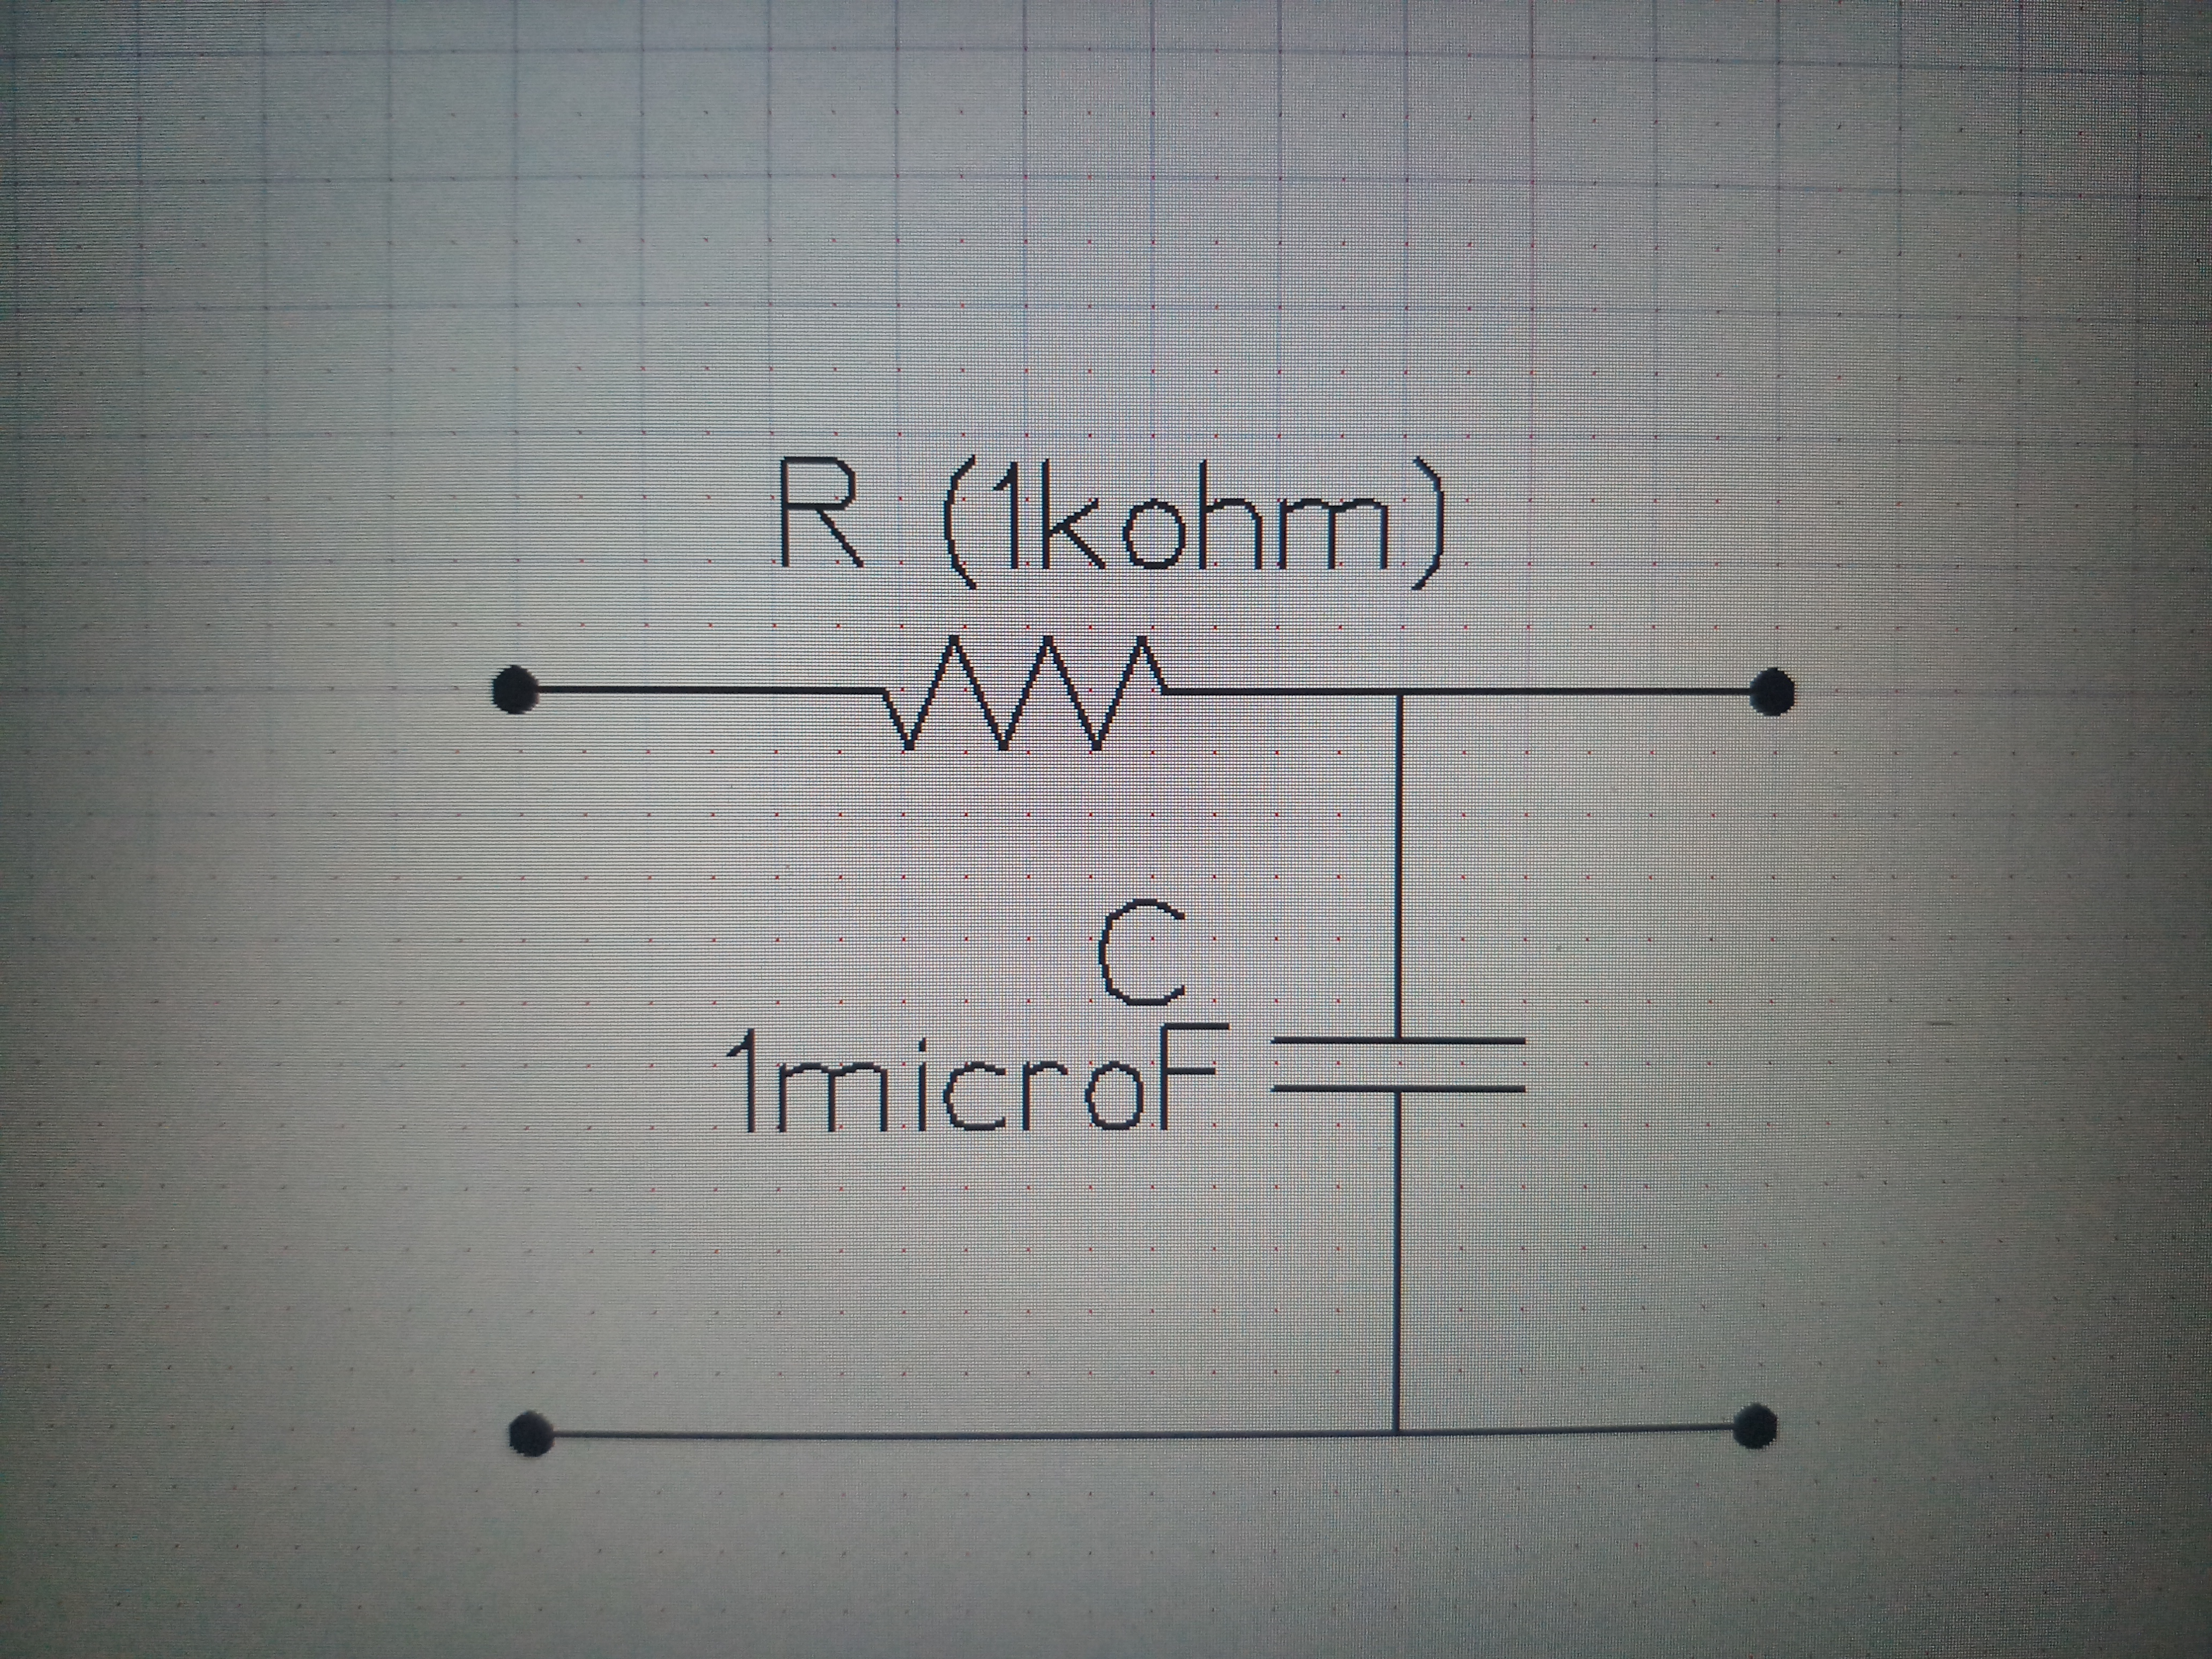
\includegraphics[width = 0.25\linewidth, trim = {0 0 0 0}, clip]{Circuit_Diagram.png}
	\caption{Equivalent Circuit Diagram}
\end{figure}

We can plot the I-V Characteristics from the data calculated as shown:

\begin{figure}[H]
	\begin{center}	
	\begin{subfigure}[b]{\linewidth}
	   	\includegraphics[width = \linewidth, trim = {0 0 0 0}, clip]{IV13.png}
		\caption{Terminal 1 / Terminal 3}
	\end{subfigure}\\
	\end{center}
	\caption{I-V Characteristics of Unknown Device}
\end{figure}
\begin{figure}[H]
	\begin{center}
	\begin{subfigure}[b]{0.85\linewidth}
	   	\includegraphics[width = \linewidth, trim = {0 0 0 0}, clip]{IV23.png}
		\caption{Terminal 2 / Terminal 3}
	\end{subfigure}\\
	\end{center}
	\begin{center}
	\begin{subfigure}[b]{0.85\linewidth}
	   	\includegraphics[width = \linewidth, trim = {0 0 0 0}, clip]{IV12.png}
		\caption{Terminal 1 / Terminal 2}
	\end{subfigure}\\
	\end{center}
\end{figure}

\end{document}
